%
% teil3.tex -- Beispiel-File für Teil 3
%
% (c) 2020 Prof Dr Andreas Müller, Hochschule Rapperswil
%
% !TEX root = ../../buch.tex
% !TEX encoding = UTF-8
%
\section{Anwendungsbeispiel
\label{openfoam:section:Anwendungsbeispiel}}
\kopfrechts{Anwendungsbeispiel}
Wie wir gesehen haben, kann OpenFOAM, mit genügend Geduld, alles. 
Wir werden jetzt an einem praktischen Beispiel zeigen, wie man eine eigene Simulation erstellt.

Für ein anschauliches Beispiel haben wir ein Objekt gewählt, dass alle Studenten der OST-Rapperswil kennen: den Campus selbst.
Das Ziel der Simulation ist, zu sehen, wie der Wind um die Gebäude strömt und mit ihnen interagiert.

Als erstes brauchen wir ein geeignetes 3d Objekt, in unserem Fall wurden die Gebäude in Onshape erstellt.
%hint, open foam arbeite in Meter, wenn das Objekt in mm exportiert wurde, faktor 1000 zu gross
Dieses 3D file bildet die Grundlage unsere Simulation.

\subsubsection{Mesh generating\label{openfoam:section:Mesh generating}}
Der grundlegende Schritt einer jeder Simulation ist, die reale, analoge Welt in eine diskrete Welt zu überführen.
Mithilfe der \textbf{snappyHexMesh} funktion wird das 3d-Objekt in disktrete Zellen unterteilt. Je mehr Zellen desto genauer
wird die Simulation, desto grösser jedoch der Aufwand für die Simulation. Diese Abwägung, Qualität vs. Aufwand, muss vom Auftraggeber definiert werden.
Die Zellen können eine freie Form annehmen, oft wird in einem ersten Durchlauf der Simulationsraum grob in Quader aufgeteilt (\ref{fig:snappygrobbild}),
in folgenden Schritten wird die Annäherung and das Grundmodell immer besser (\ref{fig:snappyfeinbild}).
%TODO xxxxxxxxxxxxxxxxxxxxxxxxxxxxxxxxxxxxxxxxxxxxxxxxxx
\subsubsection{surfaceFeatureExtract\label{openfoam:section:surfaceFeatureExtract}}
Erstellt .eMesh datei und extrahiert alle Features des 3d Objekts für die weitere Verarbeitung.

\subsubsection{blockMesh\label{openfoam:section:blockMesh}}
Grösse der Zellen definieren wie genau und aufwendig die Simulation wird

\subsubsection{snappyHexMesh\label{openfoam:section:snappyHexMesh}}
Im dict den ort des 3d Obj und eMesh files angeben, dauert lange
%TODO xxxxxxxxxxxxxxxxxxxxxxxxxxxxxxxxxxxxxxxxxxxxxxxxxx

\begin{figure}
    \centering
    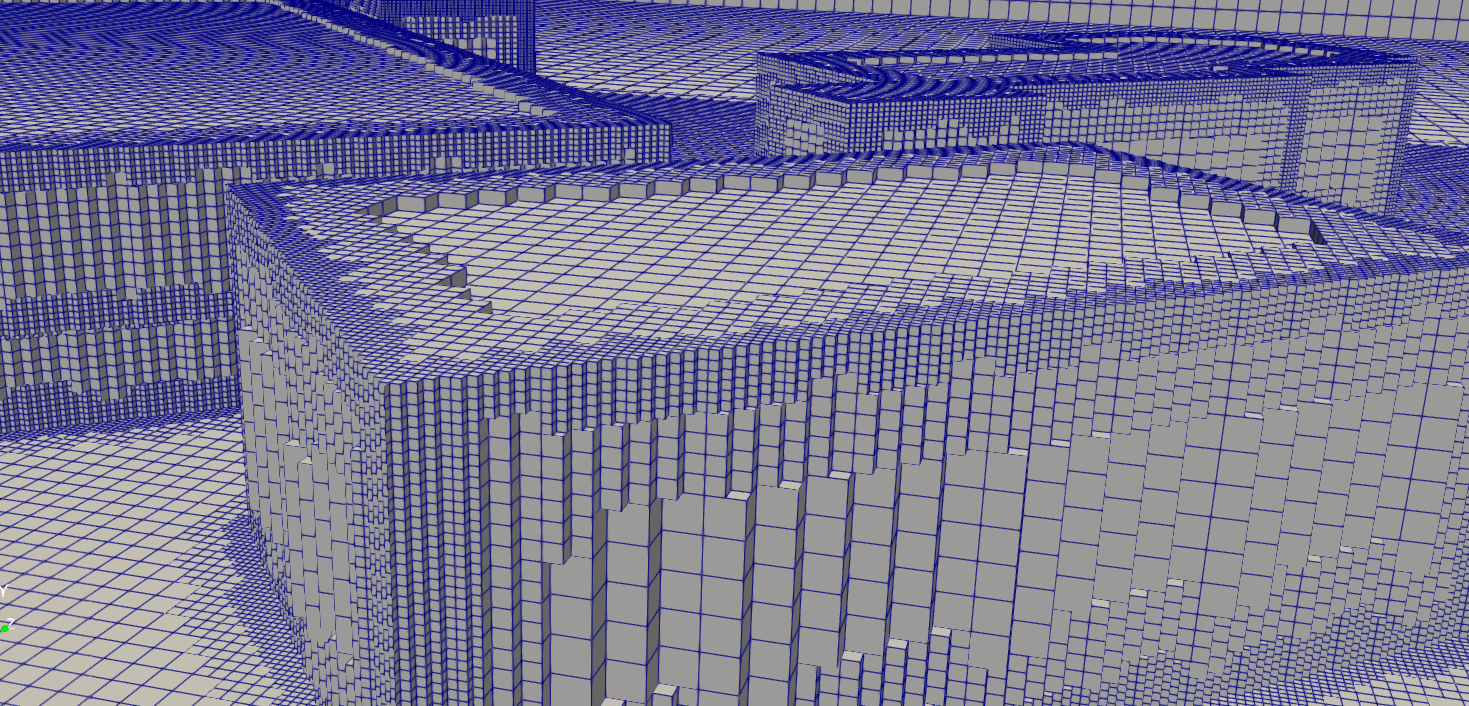
\includegraphics[width=0.55\textwidth]{papers/openfoam/Bilder/Snappy_grob.png}
    \caption{Mesh nach dem ersten Durchlauf von snappyHexMesh}
    \label{fig:snappygrobbild}
\end{figure}

\begin{figure}
    \centering
    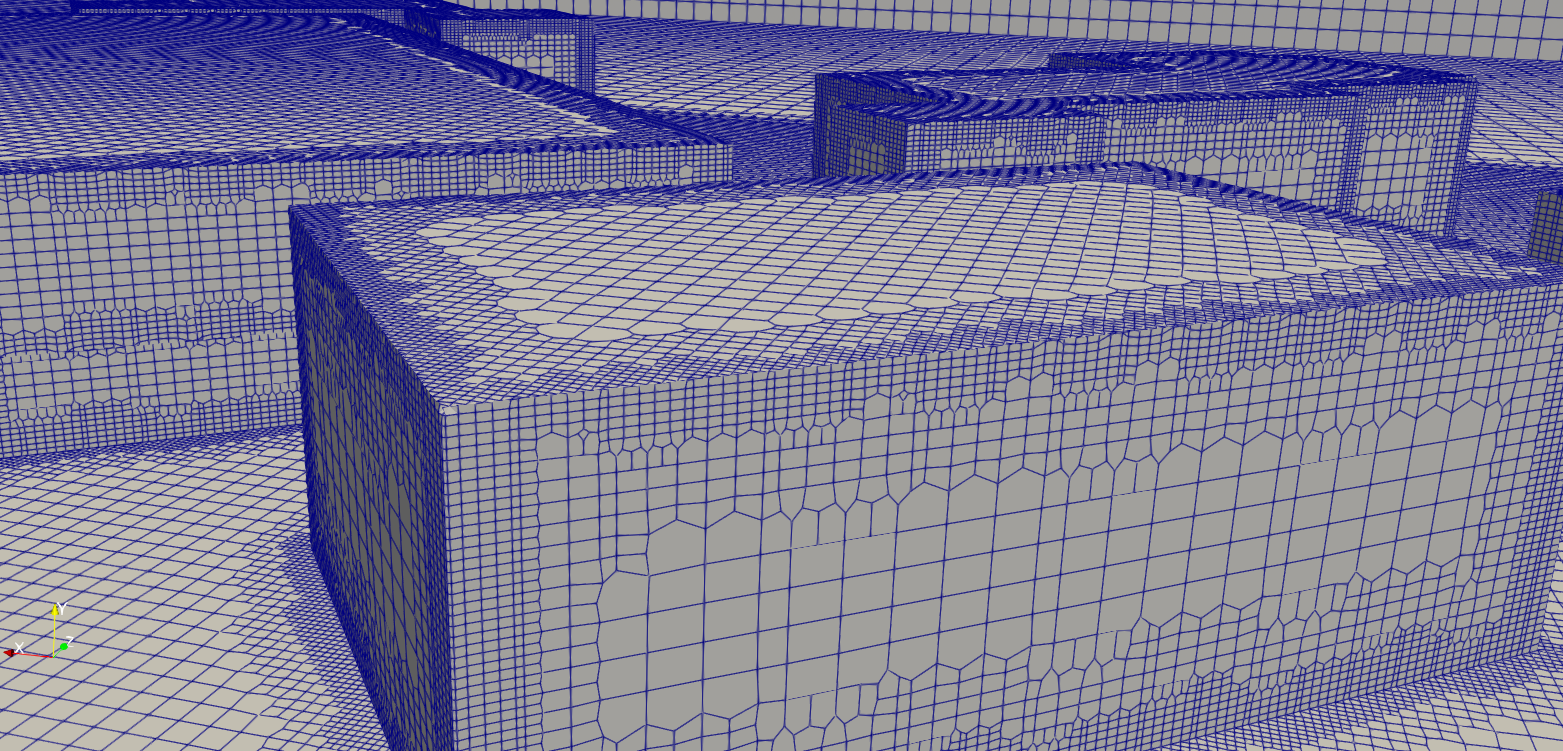
\includegraphics[width=0.55\textwidth]{papers/openfoam/Bilder/Snappy_fein.png}
    \caption{Mesh nach dem zweiten Durchlauf von snappyHexMesh}
    \label{fig:snappyfeinbild}
\end{figure}
%-------------------------------------------------------------------------------
\subsubsection{Parameter\label{openfoam:section:Parameter}}
Im folgenden einen kurzen Überblick über die wichtigsten Parameter einer OpenFOAM Simulation.

\subsubsection{Numerische Parameter\label{openfoam:section:Numerische Parameter}}
Mit den numerischen Paramter im File \textbf{controlDict} wird festgelegt:
\begin{itemize}
    \item Endzeit: Gibt an, bis zu welchem Zeitpunkt simuliert werden soll.
    \item Solver-Einstellungen: Hier wird definiert, welche numerischen Methoden verwendet werden (z.B. Diskretisierungsschemata, Iterationsverfahren) und welche Konvergenzkriterien gelten.
    \item Schreibintervall: Legt fest, wie oft während der Simulation Ergebnisse gespeichert werden.
\end{itemize}

\subsubsection{Konstante Parameter\label{openfoam:section:Konstante Parameter}}
Im \textbf{constant} Ordner werden die Transport und Turbulenz Parameter gesetzt:
\begin{itemize}
    \item Transport \textbf{transportProperties}: Welches Transportmodell verwendet wird.
    \item Turbulenzen \textbf{turbulenceProperties}: Festlegung des Simulationstyp, Reynolds-Averaged Navier-Stokes (RANS), Large Eddy Simulation (LES) oder Laminar.
\end{itemize}

\subsubsection{Anfangsbedingungen \label{openfoam:section:Anfangsbedingungen}}
Beschreibt den Zustand im ersten Schritt der Simulation. Im \textbf{0} Ordner werden folgende Faktoren bestimmt:
\begin{itemize}
    \item Geschwindigkeit und Richtung \textbf{U}: Stärke und Richtungsvektoren für jede Zelle
    \item Druckverhältnisse \textbf{p}: Skalarfeld für die Druckverteilung
    \item Dichte $\rho$: Bei kompressiblen Fluiden nötig %can't get the rho to be fat for some reason \textbf{$\rho$} doesn't work
    \item Turbulenzen \textbf{k, epsilon, nut}: In den \textbf{k, epsilon, nut} Files wird die gesamte Turbulenz im Modell beschrieben.  
\end{itemize}

%-------------------------------------------------------------------------------
\subsubsection{Simulation\label{openfoam:section:Simulation}}
In der Simulation wird nun auf jede Zelle die in den Parameter festgelegten Gleichungen angewandt. 

%TODO
Mit den folgenden Befehlen kann eine simple Simulation mit einem Tutorial Case durchgeführt werden:

%\subsubsection{Ablauf\label{openfoam:section:Ablauf}}
\begin{enumerate}
    \item surfaceFeatureExtract: Erstellt .eMesh datei und extrahiert alle Features des 3d Objekts
    \item blockMesh: Grösse der Zellen definieren wie genau und auswendig die Simulation wird
    \item snappyHexMesh: Im dict den ort des 3d Obj und eMesh files angeben, dauert lange
    \item simpleFoam: Vor dem start die startwerte von 0.orig in 1 und 2 kopieren
\end{enumerate}
%Bild Ordnerstruktur_Simuliert
%Bild vorschlag_Wind_Westen_10m_blocky?

%TODO
abschluss für nicht windows user



%TODO
\subsubsection{Postprocessing}
%\subsection{Postprocessing\label{openfoam:section:Postprocessing}}
Postprocessing ist der Prozess, bei dem die Simulationsergebnisse visualisiert und analysiert werden. 
%Bild vorschlag_Wind_Osten_5m oder Westen, evt interessant mehrere 5/10/15m


foamToVTK
paraFoam -touch, erstellt .OpenFOAM datei, welche dann mit Paraview geöffnet wird

darstellung
Paraview, navigiere zum Simulations ordner, öffne .openFOAM datei

%https://doc.openfoam.com/2306/quickstart/
%https://www.openfoam.com/documentation/user-guide Dokumentation